\newpage
\addcontentsline{toc}{chapter}{Anhang}
\pagestyle{empty}
\vspace*{7cm}
\begin{center}
{\Huge Anhang}
\end{center}
\newpage
\pagestyle{fancy}
\markboth{Anhang}{}

\setcounter{figure}{0}
\renewcommand{\thefigure}{\Roman{figure}}


\begin{figure}[h]
\centering
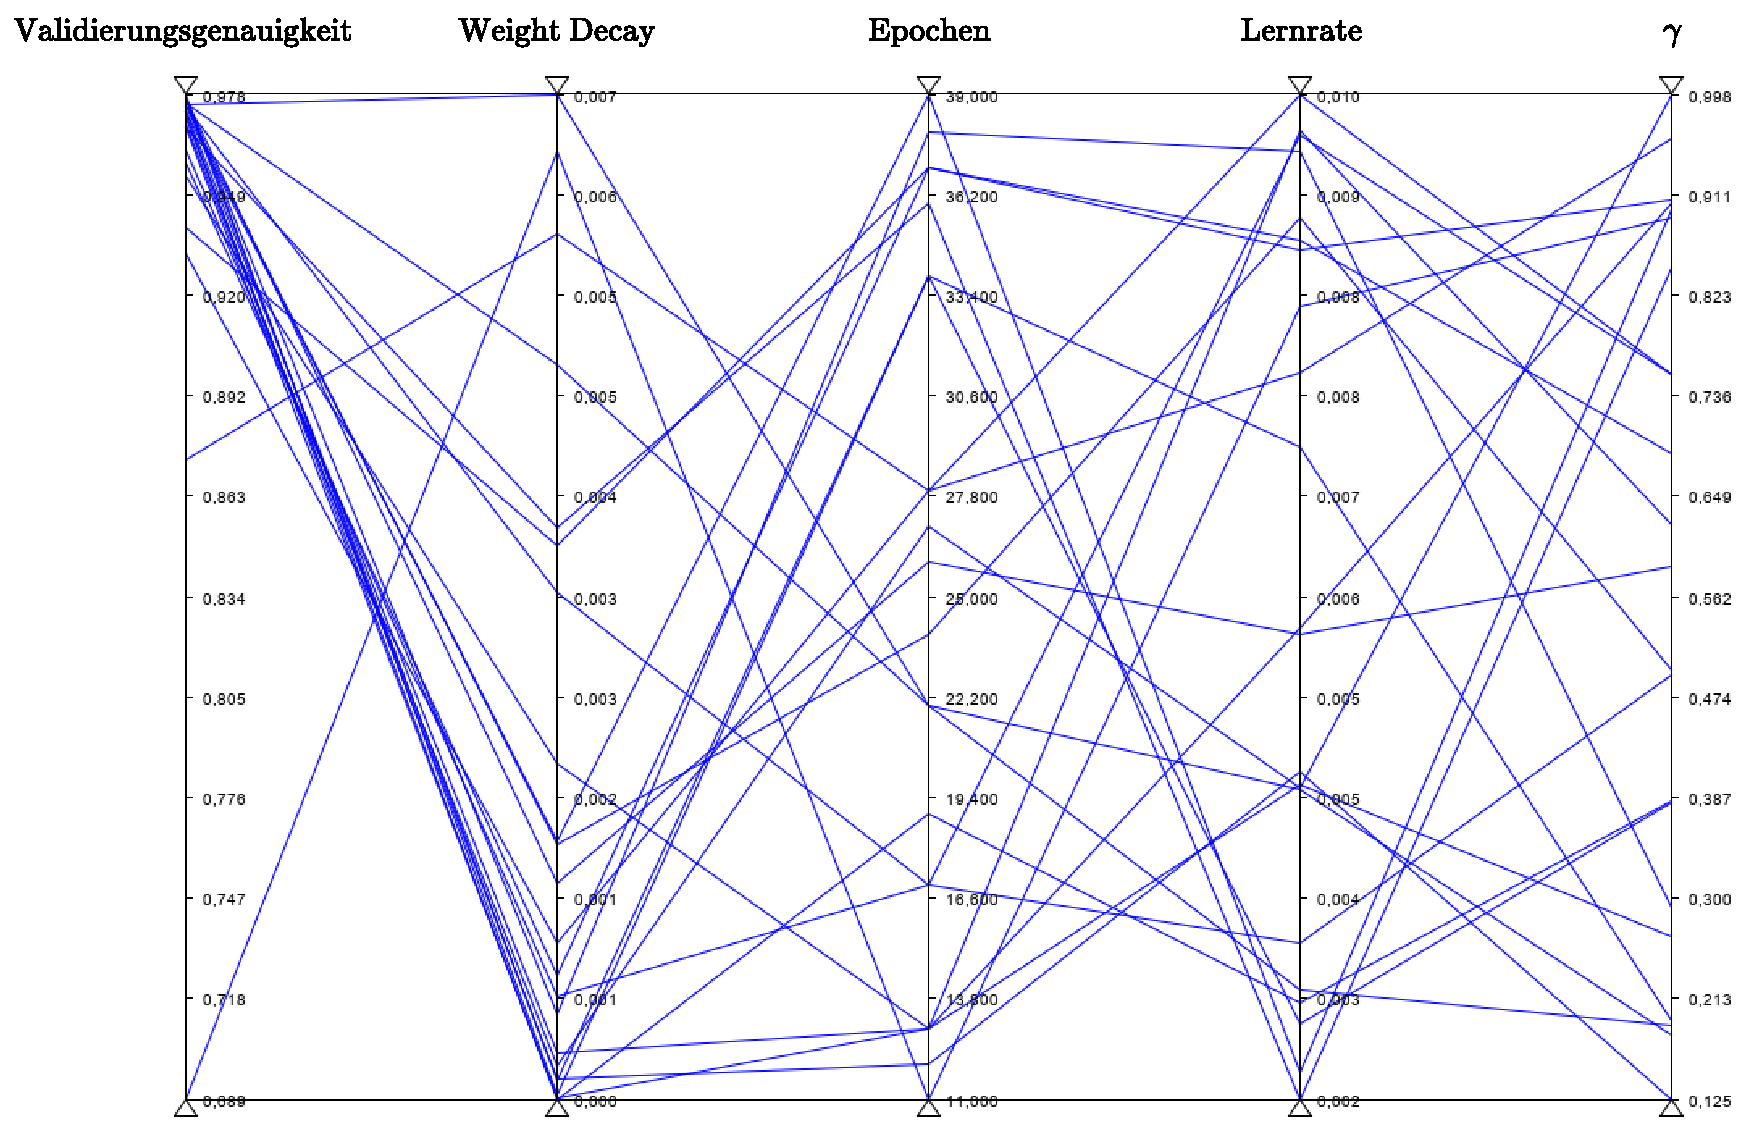
\includegraphics[scale=0.52]{NNOPT/Anhang/layer3_with_weigth_decay_finetuning}
\caption{Ergänzung zu Abb.\ref{finetuning_all} mit zusätzlicher Betrachtung des Weight Decay Parameters. Parallele Darstellung der getesteten Konfigurationen des Fine-Tunings. Jede Linie repräsentiert eine Konfiguration und die von ihr erzielte Validierungsgenauigkeit.}
\label{weight_decay_1}
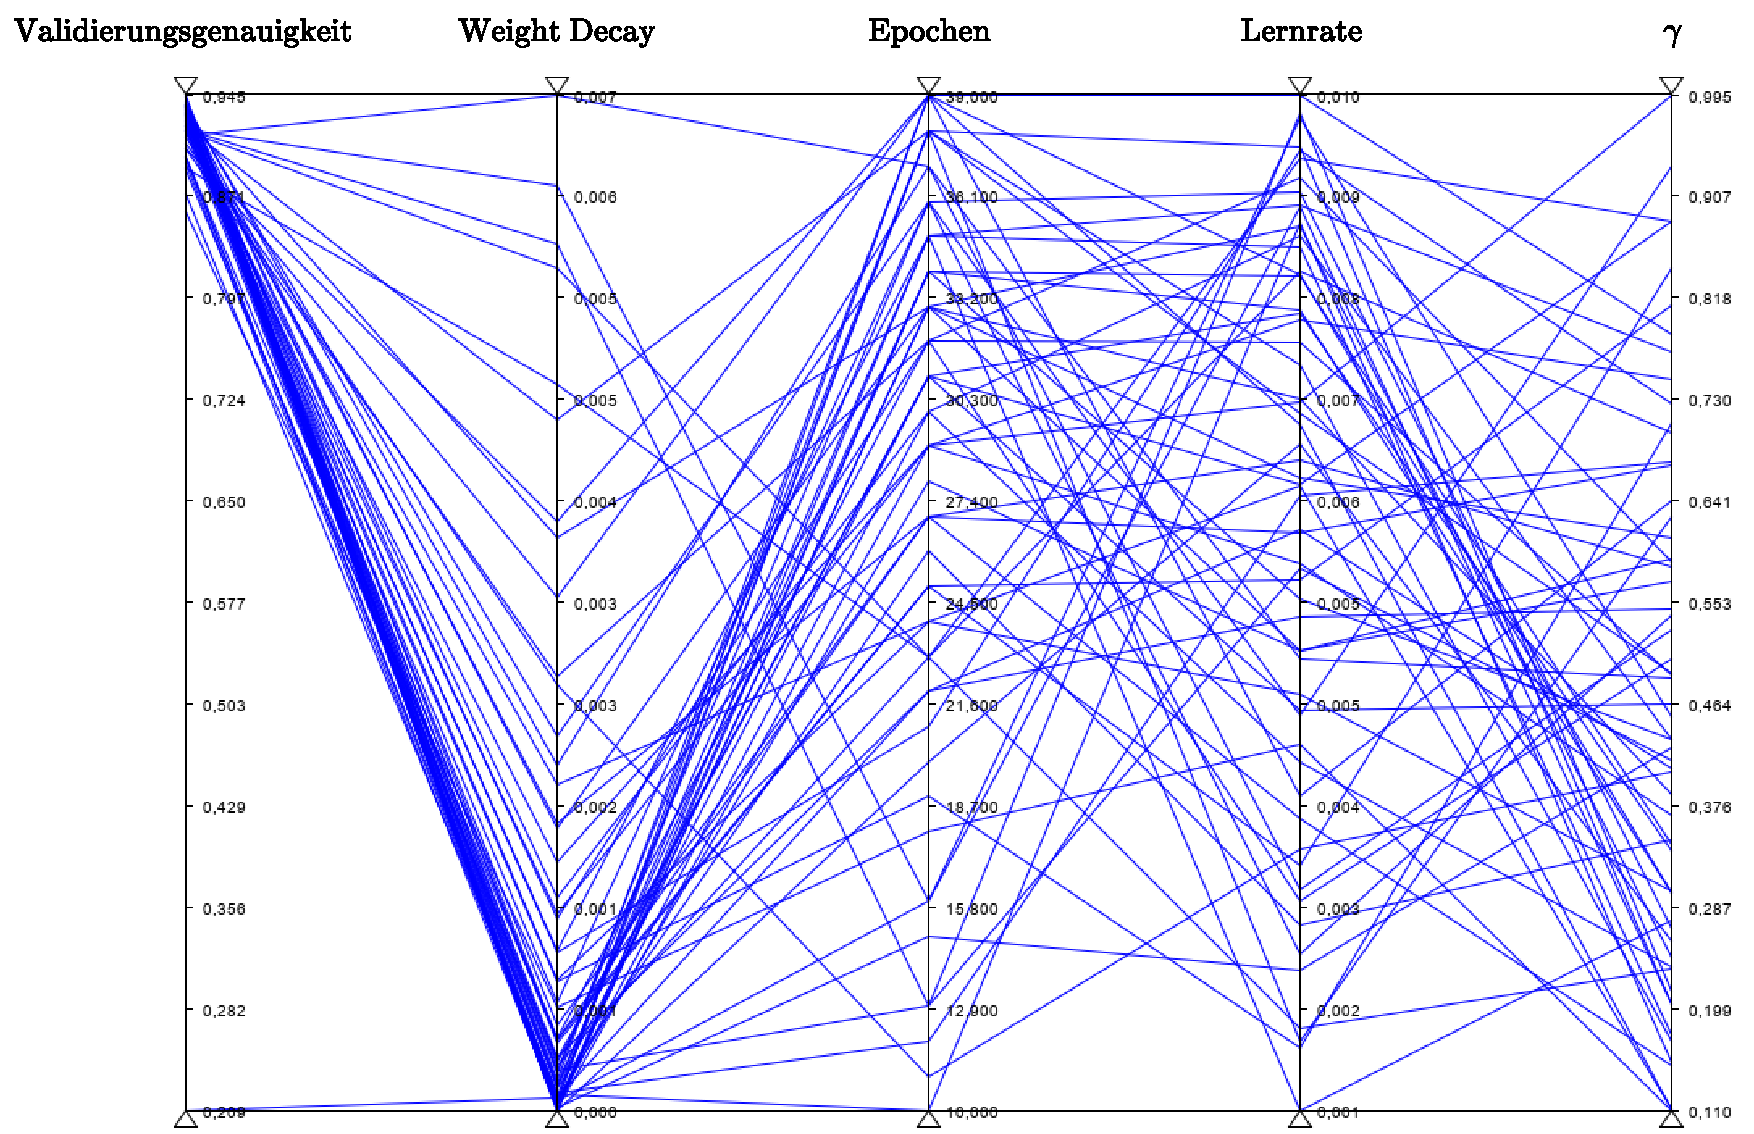
\includegraphics[scale=0.52]{NNOPT/Anhang/layer3_with_weigth_decay_attention}
\caption{Ergänzung zu Abb.\ref{attention_epochs} mit zusätzlicher Betrachtung des Weight Decay Parameters. Parallele Darstellung der getesteten Konfigurationen des Attention-Trainings. Jede Linie repräsentiert eine Konfiguration und die von ihr erzielte Validierungsgenauigkeit.}
\label{weight_decay_2}
\end{figure}

\begin{figure}[h]
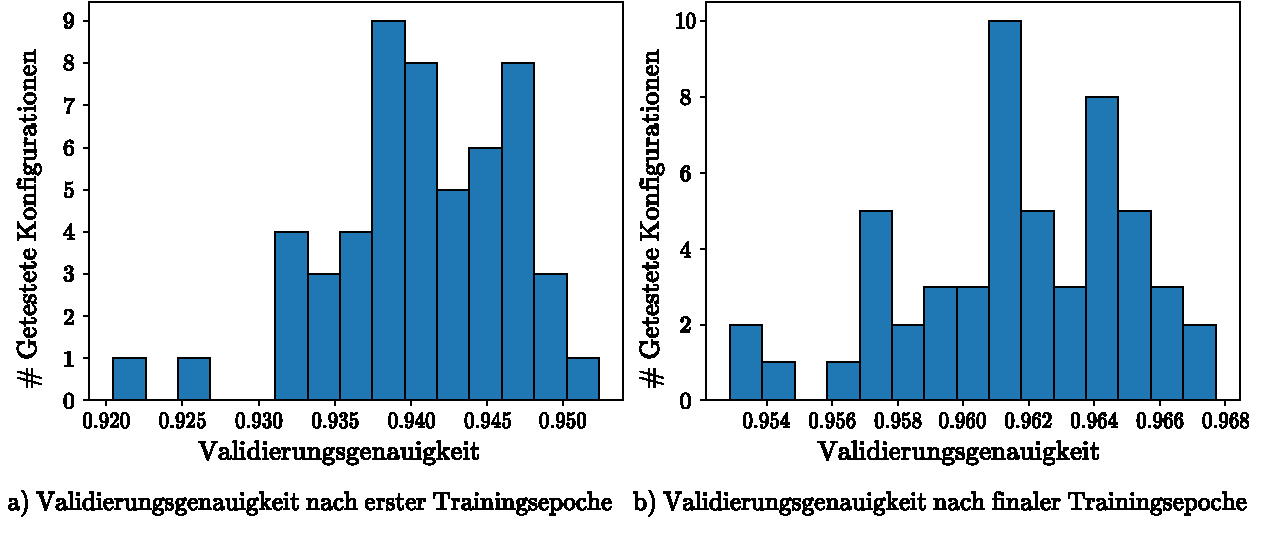
\includegraphics[scale=0.75]{NNOPT/Anhang/layer4_int_and_end_perf_attention.pdf}
\caption{Erreichte Klassifikationsgenaugikeit nach der ersten bzw. letzten Epoche des Attention-Trainings der getesteten Konfigurationen bei Verwendung von Deskriptoren aus \mbox{Block-4}. Achsenskalierung variiert.}
\label{hyperopt_layer4_1}
\end{figure}

\begin{figure}[h]
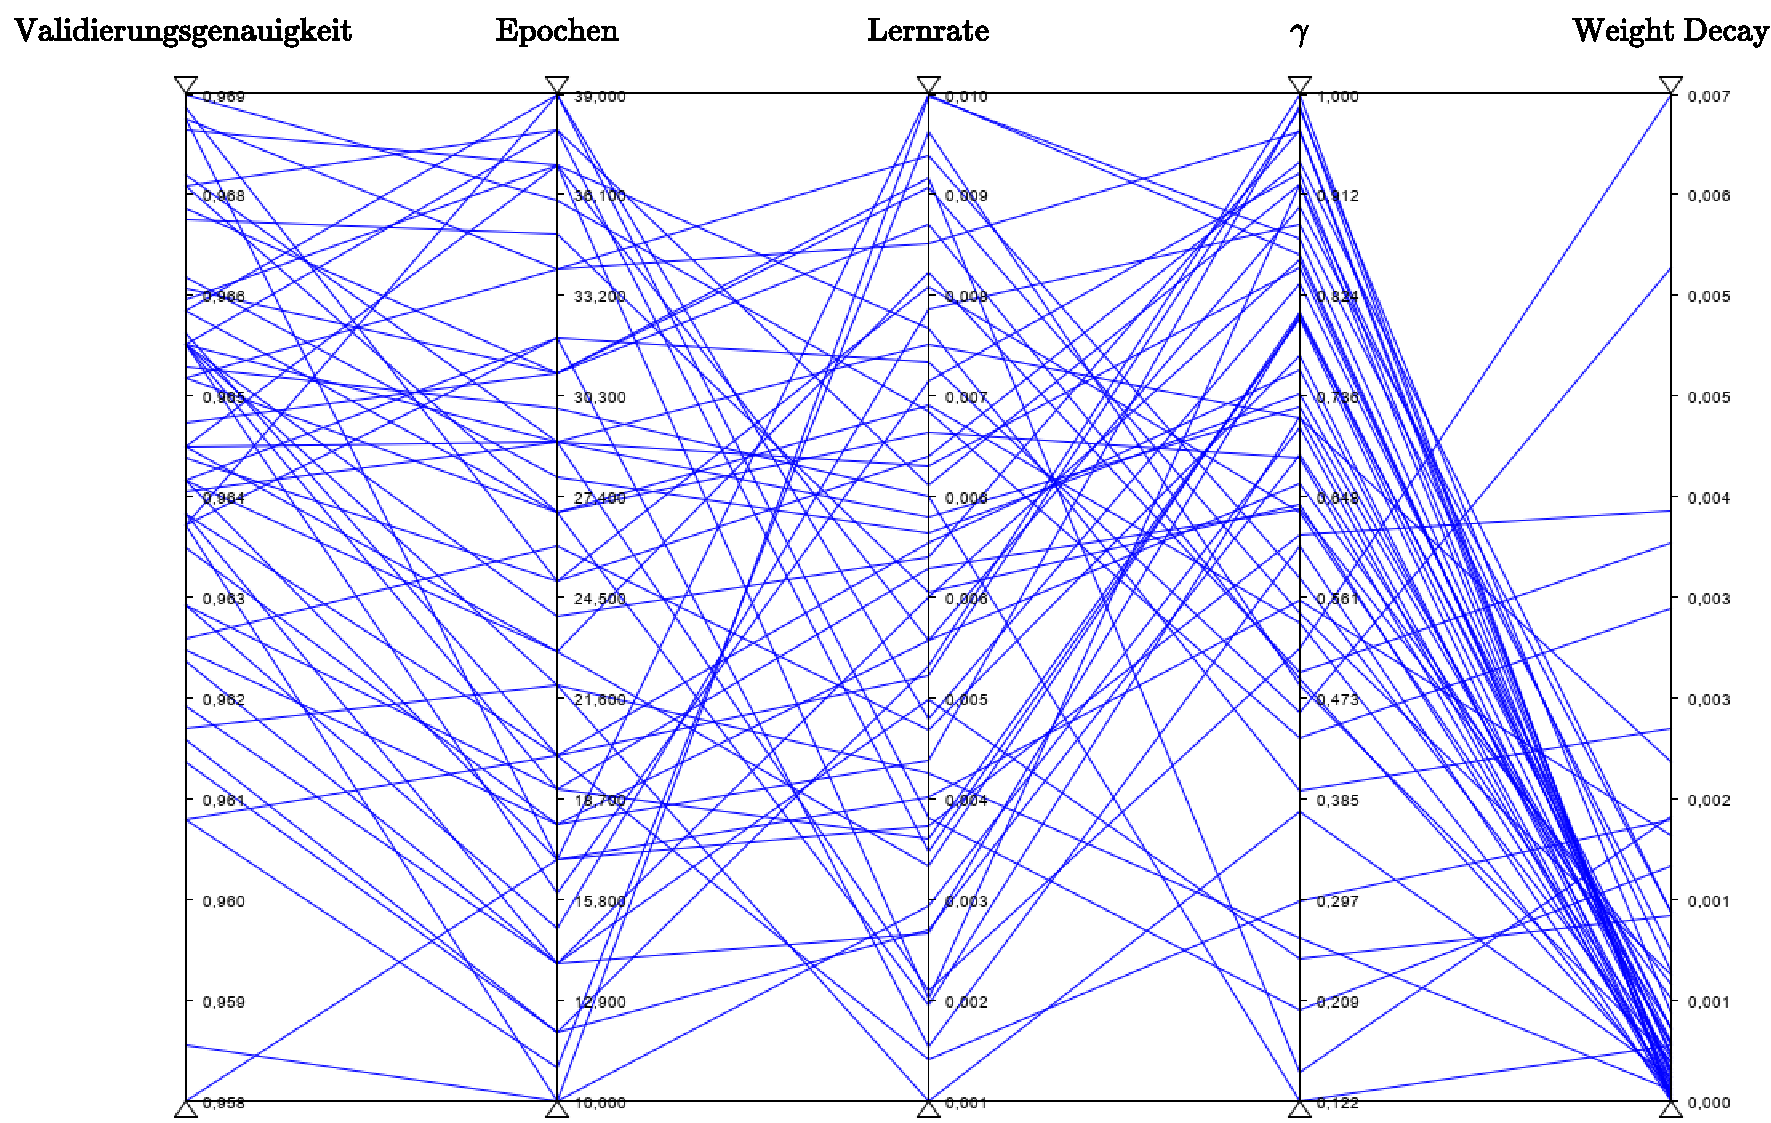
\includegraphics[scale=0.52]{NNOPT/Anhang/layer4_attention.pdf}
\caption{Parallele Darstellung der getesteten Konfigurationen des Attention-Trainings bei Verwendung von Deskriptoren aus \mbox{Block-4}. Jede Linie repräsentiert einen Konfiguration und die von ihr erzielte Validierungsgenauigkeit.}
\label{hyperopt_layer4_2}
\end{figure}
\newpage
\begin{figure}[h]
\begin{center}


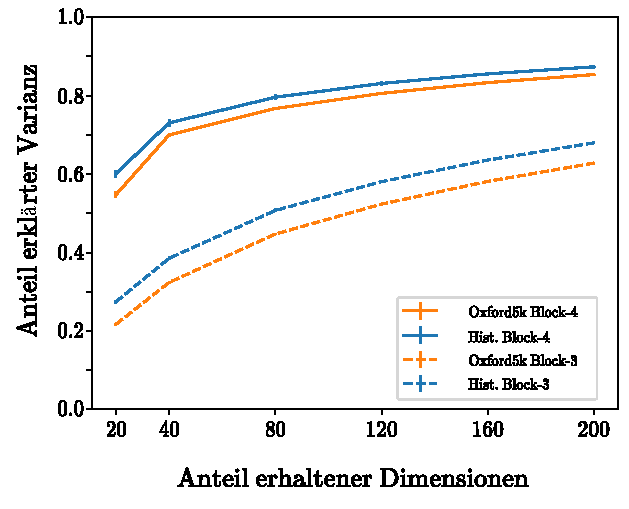
\includegraphics[scale=1.3]{NNOPT/Anhang/explained_variance_layer4}
\caption{Erklärter Anteil der Varianz nach Deskriptortransformtion durch Hauptkomponentenanalyse auf unterschiedlichen Retrievaldatensätzen bei Verwendung von unterschiedlichen Extraktionspunkten je nach Anzahl erhaltener Dimensionen. }
\label{hyperopt_layer4_3}
\end{center}

Bei Verwendung von Deskriptoren aus Block-4 kann ein deutlich größerer Anteil der Varianz in wenigen Dimensionen abgebildet werden als mit Deskriptoren aus Block-3. Dabei sind die größten Eigenwerte, die bei der Hauptkomponentenanalyse auf den Deskriptoren aus Block-4 berechnet wurden, deutlich größer als bei Verwendung von Deskriptoren aus Block-3. Das heißt, dass die ersten Hauptkomponenten/Dimensionen mehr Varianz abbilden. Zusätzlich ist die Summe der Eigenwerte bei der Analyse der Deskriptoren aus Block-4 geringer als bei Block-3. Folglich ist die Varianz zwischen den Deskriptoren aus Block-4 geringer als zwischen den Deskriptoren aus Block-3.
\end{figure}

\begin{figure}[h]
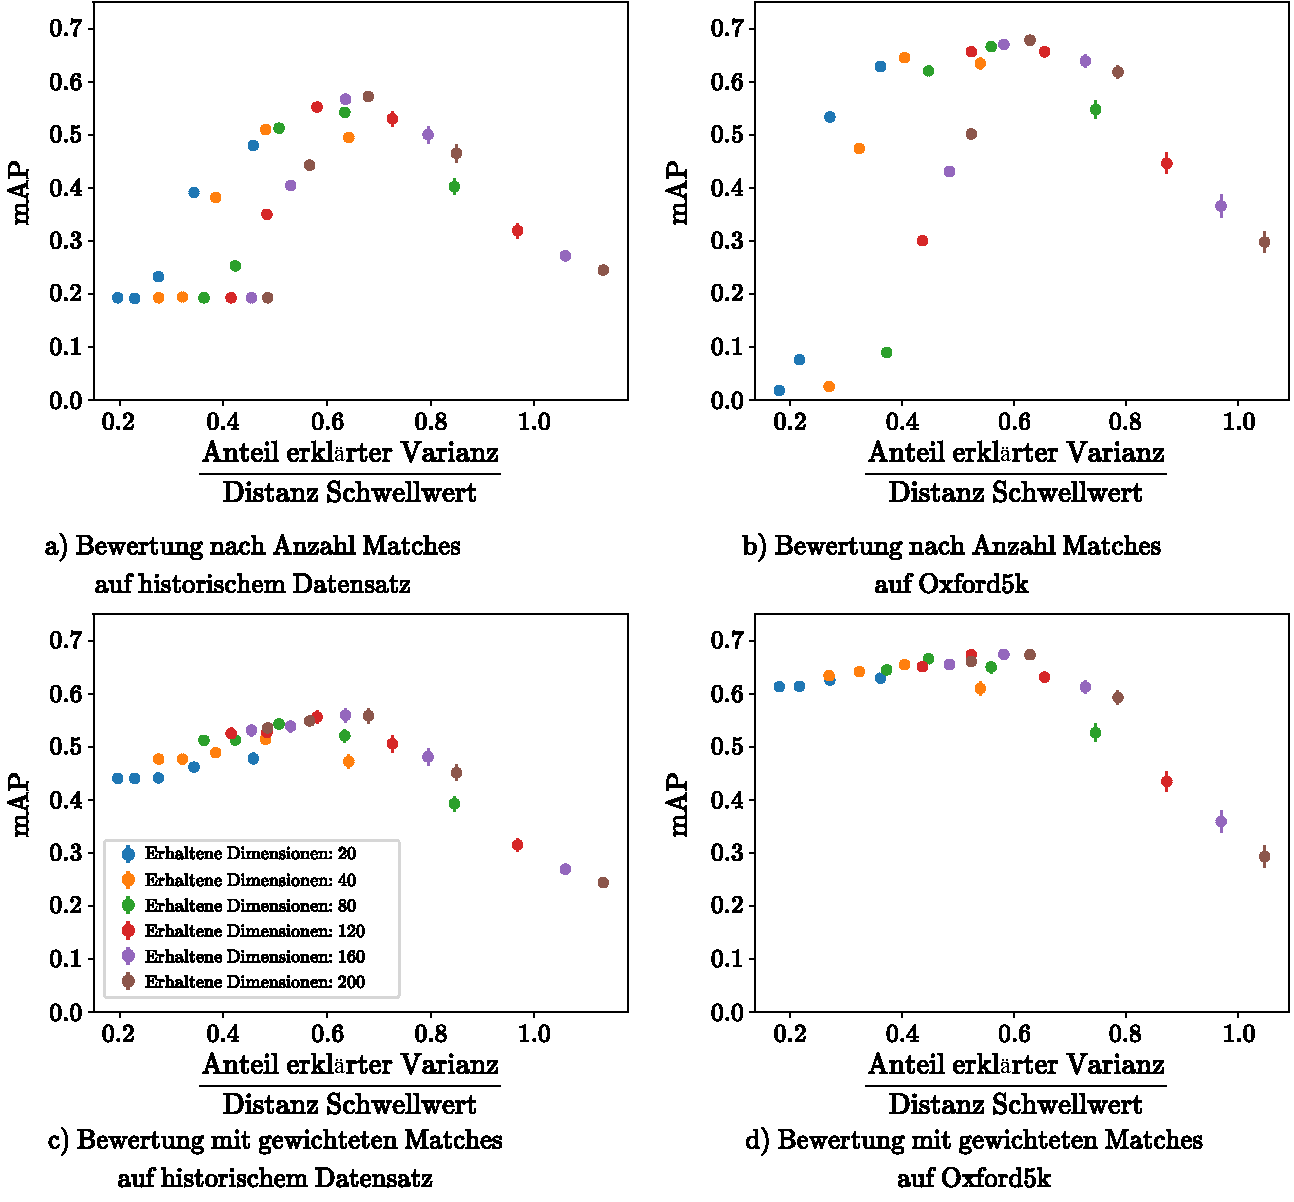
\includegraphics[scale=0.73]{mAP_var_dist_ratio_scoring_methods}
\caption{Erreichte mAP bei unterschiedlichen Verhältnissen zwischen erklärtem Varianzanteil und gewähltem Distanzschwellwert unter Verwendung alternativer Bewertungsmethoden.}
\label{mAP_var_dist_ratio_alternative_scoring}
\end{figure}